% Provenance (never printed): old seconde/premiere S material on the
% atmosphere (storms, cyclones, the energy of the water cycle) and the
% natural-hazard themes of SVT; see sources/book2/PROVENANCE.md. Tracks,
% genesis statistics and the pressure--wind relation are computed in
% figdata/grade-10/cyclones.py from IBTrACS v04r01; the surge, thunder and
% energy numbers in the same script.
\chapter{العواصف والأعاصير المدارية}\label{ch:g10:storms-and-cyclones}

ينتهي عصر يوم صيفي حار بعاصفة. تُظلم السماء، وتكنس هبة من الريح الباردة الشارع،
ويضيء وميض السحب --- فتبدأ العدّ: واحد، اثنان، ثلاثة، \ldots{} وبعد تسع ثوانٍ
يدوّي الرعد. فالعاصفة على بعد نحو ثلاثة كيلومترات. وبعد ساعة تنقضي، ويصير الهواء
باردًا نقيًا. وفوق المحيطات المدارية الدافئة، يمكن للمكونات نفسها --- هواء دافئ
رطب يصعد ويتكاثف --- أن تنتظم في عواصف من حجم آخر تمامًا: \omterm{def:g10:storms-and-cyclones:tropical-cyclone}{الأعاصير المدارية}، التي
يبلغ عرضها مئات الكيلومترات، وتدوم أيامًا، وتجلب رياحًا قوية بما يكفي لاقتلاع
الغابات، وارتفاعًا للبحر يغمر سواحل بأكملها. يتناول هذا الفصل \omterm{def:g10:storms-and-cyclones:thunderstorm}{العواصف الرعدية}
والأعاصير القمعية \omterm{def:g10:storms-and-cyclones:tropical-cyclone}{والأعاصير المدارية}، ومصدر طاقتها.

\begin{safety}
إن كنت تسمع الرعد، \omterm{def:g10:storms-and-cyclones:lightning}{فالبرق} قادر على أن يبلغك. ادخل مبنى أو سيارة مغلقة وابقَ فيها
إلى ما بعد آخر رعد بوقت طويل. ولا تحتمِ أبدًا تحت شجرة منعزلة، وابتعد عن قمم
التلال والحقول المكشوفة والماء.
\end{safety}

\begin{recall}
تُرسم الكتل الهوائية والجبهات والمنخفضات الجوية (مناطق الضغط المنخفض) والمرتفعات
الجوية على خرائط الطقس بخطوط تساوي الضغط (الكتاب 1، الصف 8). والخطر الطبيعي حدث
طبيعي يمكن أن يؤذي الناس وما يبنونه (الكتاب 1، الصف 5). وينتقل الصوت في الهواء
بنحو \qty{340}{m/s}، والضوء على الفور تقريبًا (كتب الفيزياء). والهواء الدافئ
الرطب الذي يصعد يبرد، ويتكاثف سحابًا عند مستوى تكاثفه، ويحرر \omterm{def:g10:earth-energy-budget:latent-heat}{حرارة كامنة}؛ والهواء
المشبع كثيرًا ما يكون غير مستقر
(\cref{ch:g10:why-clouds-form}).
\end{recall}

\section{العواصف الرعدية}

\begin{definition}[العاصفة الرعدية]\label{def:g10:storms-and-cyclones:thunderstorm}
\emph{العاصفة الرعدية}\index{عاصفة رعدية} عاصفة تنتجها سحابة ركام مزني، يصحبها
\omterm{def:g10:storms-and-cyclones:lightning}{برق} ورعد، وعادة زخات غزيرة وهبات من الريح، وأحيانًا بَرَد.
\end{definition}

تنمو \omterm{def:g10:storms-and-cyclones:thunderstorm}{العاصفة الرعدية} من هواء رطب غير مستقر. ففي مرحلتها الأولى يكبر ركام نحو
الأعلى، يغذيه تيار صاعد قوي؛ ويحرر التكاثف \omterm{def:g10:earth-energy-budget:latent-heat}{حرارة كامنة} تبقي الهواء الصاعد أدفأ
من محيطه. وفي مرحلة نضجها تبلغ السحابة \omterm{def:g10:why-clouds-form:stability}{الهواء المستقر} في الأعالي فتنبسط على شكل
سندان؛ وتكبر القطرات وحبات البَرَد حتى تسقط، ويجر المطر الساقط معه هواء باردًا
نحو الأسفل: إنه تيار هابط ينتشر عند الأرض على شكل جبهة هبات باردة. وفي مرحلتها
الأخيرة يستولي التيار الهابط على السحابة كلها، فيقطع الإمداد بالهواء الدافئ
الرطب، وتفرغ العاصفة مطرها حتى تنطفئ.

\begin{omfigure}
\begin{tikzpicture}[font=\footnotesize, >={Stealth[length=2mm]}]
  \foreach \dx/\title in {0/{أولًا: النمو}, 4.6/{ثانيًا: النضج}, 9.2/{ثالثًا: التبدد}}
    \node[anchor=north] at (\dx+1.6,-0.15) {\title};
  \draw[thick, black!60] (-0.3,0) -- (12.9,0);
  % stage 1: a tall cumulus
  \pic[scale=1.4, transform shape] at (1.6,1.2) {puffycloud};
  \pic[scale=1.1, transform shape] at (1.6,2.0) {puffycloud};
  \foreach \x in {1.2,1.6,2.0} \draw[->, thick, omThm!80!black] (\x,0.2) -- (\x,2.6);
  % stage 2: cumulonimbus with anvil
  \fill[black!8, draw=black!50] (5.0,1.0) -- (4.9,4.0) -- (4.2,4.4) -- (8.0,4.6) -- (7.4,4.0) -- (7.2,1.0) -- cycle;
  \draw[->, thick, omThm!80!black] (5.5,0.2) -- (5.5,4.2);
  \draw[->, thick, omThm!80!black] (5.9,0.2) -- (5.9,4.2);
  \draw[->, thick, omDef!80!black] (6.7,3.4) -- (6.7,0.3) -- (7.6,0.3);
  \foreach \x in {6.4,6.85,7.05} \draw[omDef!50] (\x,0.95) -- (\x-0.1,0.1);
  \node[anchor=west, align=left] at (8.0,4.6) {سندان};
  \node[anchor=west, align=left, omDef!80!black] at (7.65,0.45) {جبهة الهبات};
  % stage 3: dissipating
  \fill[black!8, draw=black!50] (9.7,1.2) -- (9.6,3.6) -- (9.0,4.0) -- (12.6,4.1) -- (12.0,3.6) -- (11.8,1.2) -- cycle;
  \foreach \x in {10.3,10.9,11.5} \draw[->, thick, omDef!80!black] (\x,3.2) -- (\x,0.3);
  \foreach \x in {10.6,11.2} \draw[omDef!50] (\x,1.15) -- (\x-0.1,0.1);
  % legend
  \draw[->, thick, omThm!80!black] (0,5.0) -- (0,5.5); \node[anchor=west] at (0.1,5.25) {تيار صاعد دافئ};
  \draw[->, thick, omDef!80!black] (3.2,5.5) -- (3.2,5.0); \node[anchor=west] at (3.3,5.25) {تيار هابط بارد};
\end{tikzpicture}

{\small مراحل \omterm{def:g10:storms-and-cyclones:thunderstorm}{العاصفة الرعدية} الثلاث (رسم تخطيطي، بغير مقياس): ركام نامٍ تغذيه
التيارات الصاعدة؛ والركام المزني الناضج، بسندانه وتياره الصاعد وتيار هابط يجره
المطر؛ والعاصفة المتبددة، وكلها تيار هابط.}
\end{omfigure}

داخل السحابة، تفصل التصادمات بين جسيمات الجليد التي يحملها الهواء صعودًا وهبوطًا
شحنات كهربائية: فتُشحن السحابة، عادةً بشحنة سالبة في أسفلها وموجبة في أعلاها،
وتكتسب الأرض تحتها شحنة خاصة بها.

\begin{definition}[البرق]\label{def:g10:storms-and-cyclones:lightning}
\emph{البرق}\index{برق} شرارة كهربائية هائلة تفرّغ المناطق المشحونة من العاصفة،
داخل السحابة، أو بين السحب، أو بين السحابة والأرض. وهو يسخّن قناة ضيقة من الهواء
فجأة إلى حد يتمدد معه الهواء بصدمة: وصوت هذا التمدد هو \emph{الرعد}.
\end{definition}

\begin{omfigure}
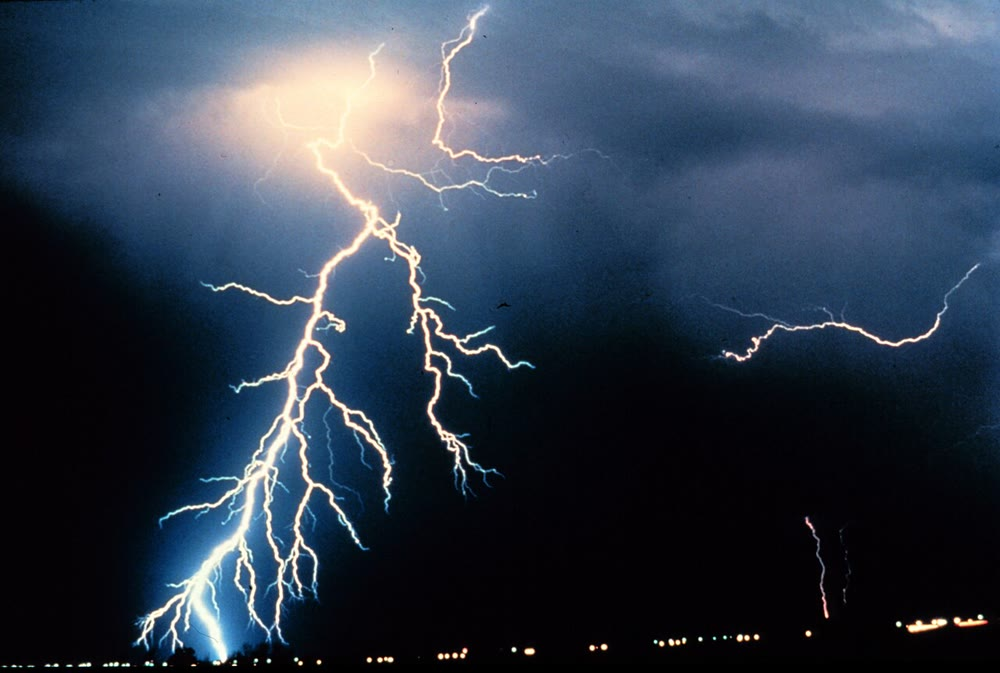
\includegraphics[width=0.62\linewidth]{images/book2/g10-noaa-lightning.jpg}

{\small ضربات \omterm{def:g10:storms-and-cyclones:lightning}{برق}، بين السحب ومن السحابة إلى الأرض، في أثناء \omterm{def:g10:storms-and-cyclones:thunderstorm}{عاصفة رعدية} ليلية.
الصورة: س.~كلارك، المختبر الوطني للعواصف الشديدة التابع للإدارة الوطنية للمحيطات
والغلاف الجوي (ملك عام).}
\end{omfigure}

تجد الأقمار الصناعية التي تحصي ومضات الضوء فوق الكوكب كله نحو 1.4 مليار ومضة \omterm{def:g10:storms-and-cyclones:lightning}{برق}
في السنة، أي 44 في كل ثانية.
% ledger: christian:flash-rate

\begin{method}[بعد العاصفة من الوميض إلى الرعد]\label{met:g10:storms-and-cyclones:distance}
\begin{enumerate}
  \item يصل ضوء الوميض فورًا عمليًا؛ أما الرعد فينتقل بسرعة الصوت، نحو
        \qty{343}{m/s} عند
        \qty{20}{\degreeCelsius}.
  \item عُدّ الثواني $t$ بين الوميض والرعد.
  \item البعد هو $343\,t$ مترًا: نحو \qty{1}{km} لكل
        ثلاث ثوانٍ.
\end{enumerate}
\end{method}
% ledger: const:R, earth:Mmol (speed of sound computed in figdata/grade-10/cyclones.py)

\section{الأعاصير القمعية}

\begin{definition}[الإعصار القمعي]\label{def:g10:storms-and-cyclones:tornado}
\emph{الإعصار القمعي}\index{إعصار قمعي} عمود من الهواء يدور بعنف ويلامس الأرض،
متدلٍّ من قاعدة ركام مزني.
\end{definition}

تأتي أقوى الأعاصير القمعية من \emph{الخلايا الفائقة}، وهي \omterm{def:g10:storms-and-cyclones:thunderstorm}{عواصف رعدية} يدور
تيارها الصاعد كله. \omterm{def:g10:storms-and-cyclones:tornado}{والإعصار القمعي} صغير وقصير العمر: يبلغ عرضه عادةً بضع مئات من
الأمتار، ويدوم دقائق، ومتوسط طول مساره نحو
\qty{5.6}{km}. لكن رياحه هي الأقوى عند سطح الأرض: فقد قاس رادار متنقل نحو
\qty{135}{m/s} (قرابة \qty{480}{km/h}) فوق الأرض في \omterm{def:g10:storms-and-cyclones:tornado}{إعصار قمعي} في أوكلاهوما في
مايو 1999. وفي الولايات المتحدة أعاصير قمعية أكثر من أي بلد آخر، نحو 1200 في
السنة؛ ومن المناطق الأخرى التي تكثر فيها البراري الكندية، وبنغلاديش، وشمال
الأرجنتين وجنوب البرازيل، وبريطانيا.
% ledger: spc:tornado

\begin{omfigure}
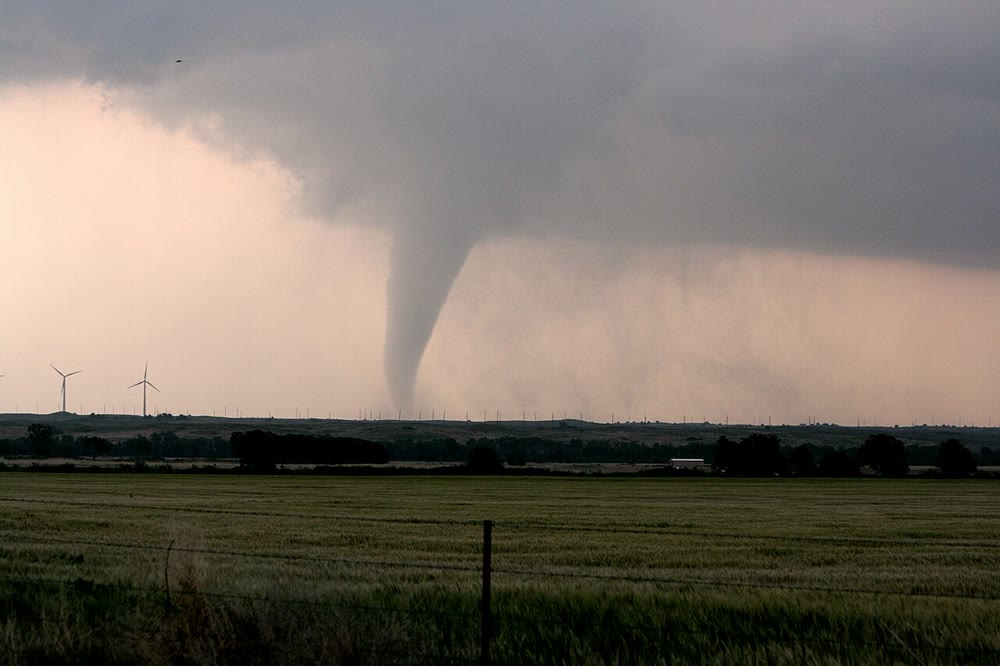
\includegraphics[width=0.62\linewidth]{images/book2/g10-noaa-tornado-kansas.jpg}

{\small \omterm{def:g10:storms-and-cyclones:tornado}{إعصار قمعي} فوق سهول كانساس، مايو 2008: يتدلى القمع من قاعدة سحابة العاصفة.
الصورة: شون وو، المختبر الوطني للعواصف الشديدة التابع للإدارة الوطنية للمحيطات
والغلاف الجوي (ملك عام).}
\end{omfigure}

\section{الأعاصير المدارية}

\begin{definition}[الإعصار المداري؛ العين؛ جدار العين]\label{def:g10:storms-and-cyclones:tropical-cyclone}
\emph{الإعصار المداري}\index{إعصار مداري} عاصفة يبلغ عرضها مئات الكيلومترات،
تتكون فوق بحر مداري دافئ حول مركز ضغط منخفض، رياحها تلتف حلزونيًا نحو المركز
وتحيط بها أشرطة من \omterm{def:g10:storms-and-cyclones:thunderstorm}{العواصف الرعدية}. وحين تبلغ رياحها المستديمة \num{64}~عقدة، أي
نحو \qty{119}{km/h}، يُسمّى «هاريكين» في المحيط الأطلسي وشرق المحيط الهادئ،
و«تيفون» في غرب المحيط الهادئ، و«سيكلون» فحسب في المحيط الهندي وجنوب المحيط
الهادئ؛ ونسمّيه في هذا الكتاب إعصارًا. ومركزه الهادئ الخالي من السحب تقريبًا هو
\emph{العين}\index{عين الإعصار}؛ وحلقة \omterm{def:g10:storms-and-cyclones:thunderstorm}{العواصف الرعدية} الشاهقة المحيطة بها، حيث
تكون الرياح على أشدها، هي \emph{جدار العين}\index{جدار العين}.
\end{definition}
% ledger: nhc:sshws

\begin{omfigure}
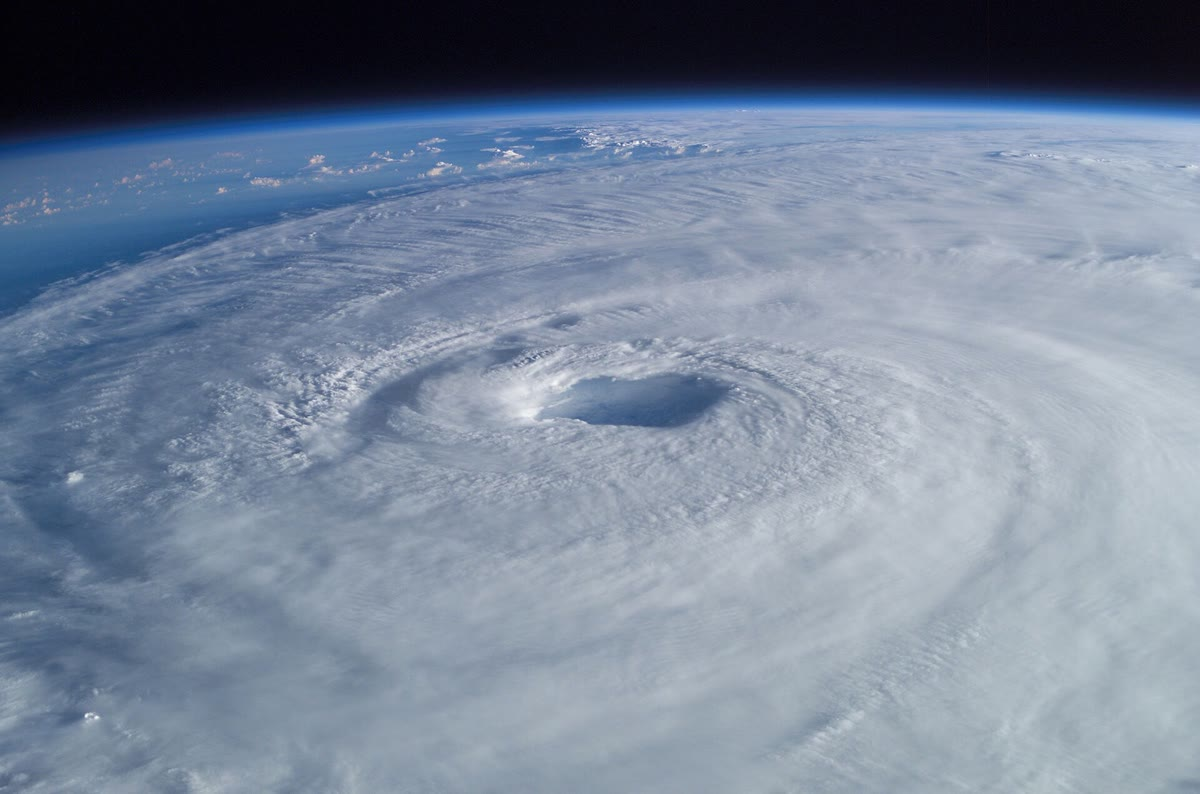
\includegraphics[width=0.78\linewidth]{images/book2/g10-nasa-hurricane-isabel.jpg}

{\small الإعصار إيزابيل، 15 سبتمبر 2003، كما صوّره رائد فضاء من محطة الفضاء
الدولية: \omterm{def:g10:storms-and-cyclones:tropical-cyclone}{العين}، \omterm{def:g10:storms-and-cyclones:tropical-cyclone}{وجدار العين}، وحلزون السحب المحيط بهما. الصورة: مايك ترينشارد،
مختبر علوم الأرض وتحليل الصور، مركز جونسون الفضائي التابع لناسا (ملك
عام).}
\end{omfigure}

قرب سطح البحر يتدفق الهواء الرطب نحو الضغط المنخفض في المركز. ودوران الأرض يحرف
الهواء المتحرك نحو اليمين في نصف الكرة الشمالي: فبدلًا من أن يتجه الهواء مباشرة
إلى المركز، يدور حوله، عكس اتجاه عقارب الساعة إذا نُظر إليه من الأعلى (ومع
اتجاهها في نصف الكرة الجنوبي). وقرب المركز يصعد في \omterm{def:g10:storms-and-cyclones:tropical-cyclone}{جدار العين}، ويتكاثف، ثم يتدفق
خارجًا من قمة العاصفة. وفي \omterm{def:g10:storms-and-cyclones:tropical-cyclone}{العين} يهبط قليل من الهواء فيسخن ويجف: فتصفو
السماء.

\begin{omfigure}
\begin{tikzpicture}[font=\footnotesize, >={Stealth[length=2mm]}]
  \fill[omDef!25] (-6,-0.4) rectangle (6,0);
  \node[anchor=north, omDef!80!black] at (0,-0.05) {بحر دافئ};
  % rain bands
  \foreach \x/\h in {-5.0/1.6, -3.9/2.2, 3.9/2.2, 5.0/1.6}
    \fill[black!10, draw=black!45] (\x-0.35,0.4) -- (\x-0.3,\h) .. controls (\x-0.15,\h+0.35) and (\x+0.15,\h+0.35) .. (\x+0.3,\h) -- (\x+0.35,0.4) -- cycle;
  % eyewall towers and outflow canopy
  \fill[black!14, draw=black!50] (-2.4,0.4) -- (-2.5,4.0) -- (-5.8,4.3) -- (-5.6,4.7) -- (-1.0,4.9) -- (-0.75,4.0) -- (-0.8,0.4) -- cycle;
  \fill[black!14, draw=black!50] (2.4,0.4) -- (2.5,4.0) -- (5.8,4.3) -- (5.6,4.7) -- (1.0,4.9) -- (0.75,4.0) -- (0.8,0.4) -- cycle;
  % inflow, rise, outflow, eye subsidence
  \draw[->, thick, omThm!80!black] (-5.8,0.2) -- (-1.3,0.2) -- (-1.3,4.3) -- (-4.2,4.45);
  \draw[->, thick, omThm!80!black] (5.8,0.2) -- (1.3,0.2) -- (1.3,4.3) -- (4.2,4.45);
  \draw[->, thick, omDef!80!black] (0,4.3) -- (0,1.0);
  \node[anchor=south, align=center] at (0,5.0) {العين: هواء\\جاف هابط};
  \node[anchor=south east, align=right] at (-2.6,4.95) {جدار العين};
  \node[anchor=west, align=left] at (-5.95,2.9) {أشرطة\\المطر};
  \node[anchor=north, align=center] at (-3.6,0.15) {تدفق رطب نحو الداخل};
  \node[anchor=south east, align=right] at (5.8,4.95) {تدفق خارج في الأعالي};
  % plan view
  \begin{scope}[shift={(8.4,2.3)}]
    \draw[black!40] (0,0) circle (1.7);
    \foreach \a in {0,90,180,270}
      \draw[->, thick, omThm!80!black, domain=0:200, samples=30, variable=\t]
        plot ({(1.6-0.0045*\t)*cos(\a+\t)}, {(1.6-0.0045*\t)*sin(\a+\t)});
    \fill[white, draw=black!50] (0,0) circle (0.22);
    \node[anchor=north, align=center] at (0,-1.8) {منظر من الأعلى\\(نصف الكرة الشمالي)};
  \end{scope}
\end{tikzpicture}

{\small \omterm{def:g10:storms-and-cyclones:tropical-cyclone}{إعصار مداري} في مقطع عرضي (رسم تخطيطي، والارتفاع مبالغ فيه كثيرًا): يتدفق
الهواء الرطب فوق البحر الدافئ نحو الداخل، ويصعد في \omterm{def:g10:storms-and-cyclones:tropical-cyclone}{جدار العين} وفي أشرطة المطر، ثم
يتدفق خارجًا من القمة؛ ويهبط قليل من الهواء في \omterm{def:g10:storms-and-cyclones:tropical-cyclone}{العين}.
في اليمين: منظر من الأعلى في نصف الكرة الشمالي، حيث يدور التدفق الداخل
عكس اتجاه عقارب الساعة حول المركز.}
\end{omfigure}

تحتاج \omterm{def:g10:storms-and-cyclones:tropical-cyclone}{الأعاصير المدارية} إلى محيط دافئ: ماء لا تقل حرارته عند السطح عن نحو
\qty{27}{\degreeCelsius}، ويبقى دافئًا حتى عمق يقارب
\qty{46}{m}. ولا تتكون على خط الاستواء نفسه، حيث لا يعطي دوران الأرض الهواء
المتدفق أي انعطاف: فيجب أن تكون العاصفة على بعد نحو
\qty{480}{km} على الأقل من خط الاستواء كي يبدأ الدوران.
% ledger: aoml:formation

\begin{omfigure}
\begin{tikzpicture}
\begin{axis}[ommap, width=\linewidth, xtick={-180,-120,...,180}, ytick={-60,-30,0,30,60},
  ymin=-70, ymax=70, unbounded coords=jump]
\addplot[fill=omLithAlluv, draw=black!45, line width=0.2pt] table {figdata/out/shared-geo-land.dat};
\addplot[omThm!70, line width=0.25pt] table {figdata/out/grade-10-cyclones-tracks.dat};
\addplot[only marks, mark=*, mark size=0.45pt, omDef!90!black] table {figdata/out/grade-10-cyclones-genesis.dat};
\addplot[black!45, dashed, domain=-180:180] {0};
\end{axis}
\end{tikzpicture}

{\small \omterm{def:g10:storms-and-cyclones:tropical-cyclone}{الأعاصير المدارية}: مسارات كل عواصف مواسم 2015--2024 (بالأحمر)، والمكان الذي
بلغت فيه كل عاصفة من عواصف مواسم 1980--2024 قوة العاصفة المدارية أول مرة (نقاط
زرقاء). البيانات: \babelsublr{IBTrACS v04r01}، المراكز الوطنية للمعلومات البيئية
التابعة للإدارة الوطنية للمحيطات والغلاف الجوي.}
\end{omfigure}
% ledger: data:b2-ibtracs (all statistics computed in figdata/grade-10/cyclones.py)

تُظهر الخريطة القاعدة وهي تعمل. فمن \num{3888} عاصفة في 1980--2024، لم تبلغ قوة
العاصفة المدارية إلا 24 على بعد \qty{5}{\degree} من خط الاستواء. ويتكون معظمها بين
خطي العرض \qty{10}{\degree} و\qty{30}{\degree}، ثم تنجرف غربًا مع الرياح التجارية
وتنعطف بعيدًا نحو القطبين، حيث يضعفها البحر البارد. أما جنوب المحيط الأطلسي، الأبرد
والأقل ملاءمة، فلم يشهد إلا ثلاثة منها في 45 سنة. ويتكون في السنة المتوسطة نحو 87
إعصارًا مداريًا، سبعة من كل عشرة منها في نصف الكرة الشمالي، ويبلغ ما يزيد قليلًا
على نصفها قوة الإعصار.

\begin{proposition}[مصدر طاقة الإعصار المداري]\label{prop:g10:storms-and-cyclones:energy}
يستمد \omterm{def:g10:storms-and-cyclones:tropical-cyclone}{الإعصار المداري} طاقته من البحر الدافئ: \omterm{def:g10:earth-energy-budget:latent-heat}{فالحرارة الكامنة} التي يأخذها التبخر
عند سطح البحر تتحرر في \omterm{def:g10:storms-and-cyclones:tropical-cyclone}{جدار العين} وفي أشرطة المطر حين يتكاثف البخار. ويحرر الإعصار
المتوسط على هذا النحو نحو \qty{6e14}{W}؛ ولا يذهب منها إلا جزء صغير، نحو
\qty{1.5e12}{W}، إلى الطاقة الحركية لرياحه.
\end{proposition}
% ledger: aoml:energy

\begin{proof}[تعليل]
يُمطر الإعصار المتوسط \qty{1.5}{cm} في اليوم فوق دائرة نصف قطرها
\qty{665}{km}، مساحتها $\pi \times (665\,000)^2 \approx
\qty{1.39e12}{m^2}$: أي \qty{2.1e10}{m^3}، أو \qty{2.1e13}{kg}، من الماء في اليوم.
وكل كيلوغرام يتكاثف يحرر نحو \qty{2.5}{MJ}: $2.1\times10^{13}
\times 2.5\times10^6 \approx \qty{5.2e19}{J}$ في اليوم، أي
$5.2\times10^{19}/86\,400 \approx \qty{6.0e14}{W}$. أما قدرة الرياح فتقدير
مأخوذ من حقول رياح مقيسة، منقول عن المصدر نفسه.
\end{proof}

تعمل العاصفة كمحرك: حرارة تؤخذ عند سطح البحر الدافئ، وتُطرح عاليًا في الهواء العلوي
البارد، ويتحول جزء من الفرق إلى حركة الريح. ولهذا يضعف \omterm{def:g10:storms-and-cyclones:tropical-cyclone}{الإعصار المداري} سريعًا
حين ينتقل فوق اليابسة أو فوق ماء بارد: إذ يفقد إمداده بالماء المتبخر.

\section{الشدة والرياح والعرام}

\begin{definition}[سلم سافير--سيمبسون]\label{def:g10:storms-and-cyclones:scale}
\emph{سلم سافير--سيمبسون}\index{سلم سافير--سيمبسون} يصنّف الأعاصير في خمس
فئات بحسب أقصى رياحها المستديمة؛ والفئات من 3 إلى 5 هي الأعاصير
\emph{الكبرى}.
\end{definition}

\begin{center}
\small
\begin{tabular}{cccc}
\hline
الفئة & عقدة & \unit{m/s} & \unit{km/h} \\
\hline
1 & 64--82 & 33--42 & 119--153 \\
2 & 83--95 & 43--49 & 154--177 \\
3 & 96--112 & 49--58 & 178--208 \\
4 & 113--136 & 58--70 & 209--251 \\
5 & 137 أو أكثر & 70 أو أكثر & 252 أو أكثر \\
\hline
\end{tabular}
\end{center}
% ledger: nhc:sshws (m/s converted with 1 knot = 1852/3600 m/s)

كلما كان الضغط المنخفض في المركز أعمق، اشتدت الرياح التي تهب حوله: ففرق الضغط بين
المركز والمحيط هو ما يدفع الهواء نحو الداخل.

\begin{omfigure}
\begin{tikzpicture}
\begin{axis}[omrecord, width=0.86\linewidth, height=6.2cm, xmin=15, xmax=100,
  ymin=860, ymax=1015, xlabel={\foreignlanguage{arabic}{أقصى ريح مستديمة \babelsublr{(\unit{m/s})}}},
  ylabel={\foreignlanguage{arabic}{أدنى ضغط في المركز \babelsublr{(\unit{hPa})}}},
  tick label style={font=\small}, label style={font=\small}]
\foreach \w in {32.92, 42.70, 49.39, 58.13, 70.48}
  \edef\temp{\noexpand\draw[black!55, densely dashed] (axis cs:\w,860) -- (axis cs:\w,1015);}\temp
\addplot[only marks, mark=*, mark size=0.6pt, omDef!80!black, opacity=0.6] table[x=wind_ms, y=pmin_hpa] {figdata/out/grade-10-cyclones-scatter.dat};
\addplot[omThm!85!black, thick] table[x=wind_ms, y=pmin_hpa] {figdata/out/grade-10-cyclones-fit.dat};
\node[font=\scriptsize, black!60] at (axis cs:37.8,1008) {1};
\node[font=\scriptsize, black!60] at (axis cs:46.0,1008) {2};
\node[font=\scriptsize, black!60] at (axis cs:53.8,1008) {3};
\node[font=\scriptsize, black!60] at (axis cs:64.3,1008) {4};
\node[font=\scriptsize, black!60] at (axis cs:76,1008) {5};
\end{axis}
\end{tikzpicture}

{\small كل نقطة \omterm{def:g10:storms-and-cyclones:tropical-cyclone}{إعصار مداري} واحد من مواسم 2000--2024: أقوى رياحه المستديمة وأدنى
ضغط في مركزه. والخط هو أفضل خط مستقيم مطابق: أدنى بنحو \qty{1.6}{hPa} لكل متر في
الثانية إضافي. والخطوط الرمادية المتقطعة: حدود فئات \omterm{def:g10:storms-and-cyclones:scale}{سلم سافير--سيمبسون} (المرقّمة
في الأعلى). البيانات: \babelsublr{IBTrACS v04r01}، المراكز الوطنية للمعلومات
البيئية.}
\end{omfigure}
% ledger: data:b2-ibtracs, nhc:sshws (fit computed in figdata/grade-10/cyclones.py)

يعود الرقم القياسي لعواصف 1980--2024 في الأرشيف إلى الإعصار باتريسيا، قبالة ساحل
المكسيك على المحيط الهادئ في أكتوبر 2015: رياح مستديمة بلغت 185 عقدة، نحو
\qty{95}{m/s}، وضغط في المركز قدره \qty{872}{hPa}.
% ledger: data:b2-ibtracs

\begin{definition}[العرام العاصفي]\label{def:g10:storms-and-cyclones:storm-surge}
\emph{العرام العاصفي}\index{عرام عاصفي} هو ارتفاع البحر فوق مستواه المعتاد، من غير
المد، بسبب عاصفة: إذ تكدس الريح الماء على الساحل، ويسمح الضغط المنخفض للبحر بأن
ينتفخ تحت العاصفة.
\end{definition}

\begin{proposition}[الانتفاخ الضغطي]\label{prop:g10:storms-and-cyclones:bulge}
تحت عاصفة يقل ضغطها في المركز عن ضغط محيطها بمقدار $\Delta p$ هكتوباسكال، يرتفع
البحر بنحو $\Delta p$ سنتيمتر.
\end{proposition}

\begin{proof}
في العمق تحت السطح يجب أن يكون الضغط واحدًا تحت العاصفة وخارجها، وإلا لتدفق الماء.
والهواء فوق العاصفة أخف بمقدار $\Delta p$؛ وعمود من ماء البحر ارتفاعه $h$ يعوّض
ذلك إذا كان
$\rho g h = \Delta p$. ومن أجل $\Delta p = \qty{1}{hPa} = \qty{100}{Pa}$، مع
$\rho = \qty{1025}{kg/m^3}$ و$g = \qty{9.81}{m/s^2}$: $h = 100/(1025
\times 9.81) \approx \qty{0.0099}{m}$، أي نحو \qty{1}{cm}.
\end{proof}
% ledger: noaa:seawater-1025, nasa:aquarius-density, const:gn

الانتفاخ هو الجزء الأصغر من معظم العرامات: فتحت ضغط في المركز قدره
\qty{920}{hPa}، أدنى من المحيط بمقدار \qty{90}{hPa}، يبلغ نحو
\qty{0.9}{m}. والريح تتولى الباقي، دافعةً الماء نحو الشاطئ، ولا سيما فوق قاع بحر
عريض ضحل. وإذا وصل عرام من بضعة أمتار مع مدّ عالٍ، أمكنه أن يغمر السواحل المنخفضة
إلى مسافات بعيدة في الداخل.

\begin{omfigure}
\begin{tikzpicture}[font=\footnotesize, >={Stealth[length=2mm]}]
  \def\surf{(0,0) .. controls (1.5,0) and (2.2,0.5) .. (3.0,0.5) .. controls (3.8,0.5) and (4.6,0.4) .. (5.6,0.5) .. controls (7.2,0.65) and (8.8,1.0) .. (10.25,1.3)}
  \fill[omDef!20] (0,-1.6) -- \surf -- (8.8,-1.6) -- cycle;
  \draw[thick, omDef!80!black] \surf;
  \draw[black!50, dashed] (0,0) -- (9.6,0);
  \node[anchor=north west, black!60] at (0.1,-0.05) {مستوى البحر المعتاد};
  \fill[omExo!30, draw=black!60] (8.8,-1.6) -- (10.4,1.6) -- (12.4,1.7) -- (12.4,-1.6) -- cycle;
  \foreach \x in {10.9,11.7} \draw[fill=white, draw=black!60] (\x,1.63) rectangle (\x+0.45,2.03) (\x-0.05,2.03) -- (\x+0.225,2.28) -- (\x+0.5,2.03);
  \draw[<->, omThm!80!black] (3.0,0) -- (3.0,0.5);
  \node[anchor=south east, omThm!80!black, align=right] at (2.8,0.6) {انتفاخ تحت\\الضغط المنخفض};
  \draw[<->, omThm!80!black] (9.4,0) -- (9.4,1.12);
  \node[anchor=south, omThm!80!black, align=center] at (8.9,1.75) {تكدس الماء بالريح\\على الساحل};
  \foreach \y in {2.9,3.4} \draw[->, thick, black!60] (4.0,\y) -- (6.4,\y);
  \node[anchor=south] at (5.2,3.45) {ريح نحو الشاطئ};
  \node[anchor=south, align=center] at (3.0,1.9) {مركز\\العاصفة};
  \draw[black!40] (3.0,1.9) -- (3.0,0.65);
\end{tikzpicture}

{\small \omterm{def:g10:storms-and-cyclones:storm-surge}{عرام عاصفي} (رسم تخطيطي، والارتفاعات مبالغ فيها كثيرًا): يرتفع البحر بنحو
\qty{1}{cm} لكل هكتوباسكال من الضغط المنخفض تحت العاصفة، وتكدس الريح الهابة نحو
الشاطئ الماءَ على الساحل.}
\end{omfigure}

\begin{omfigure}
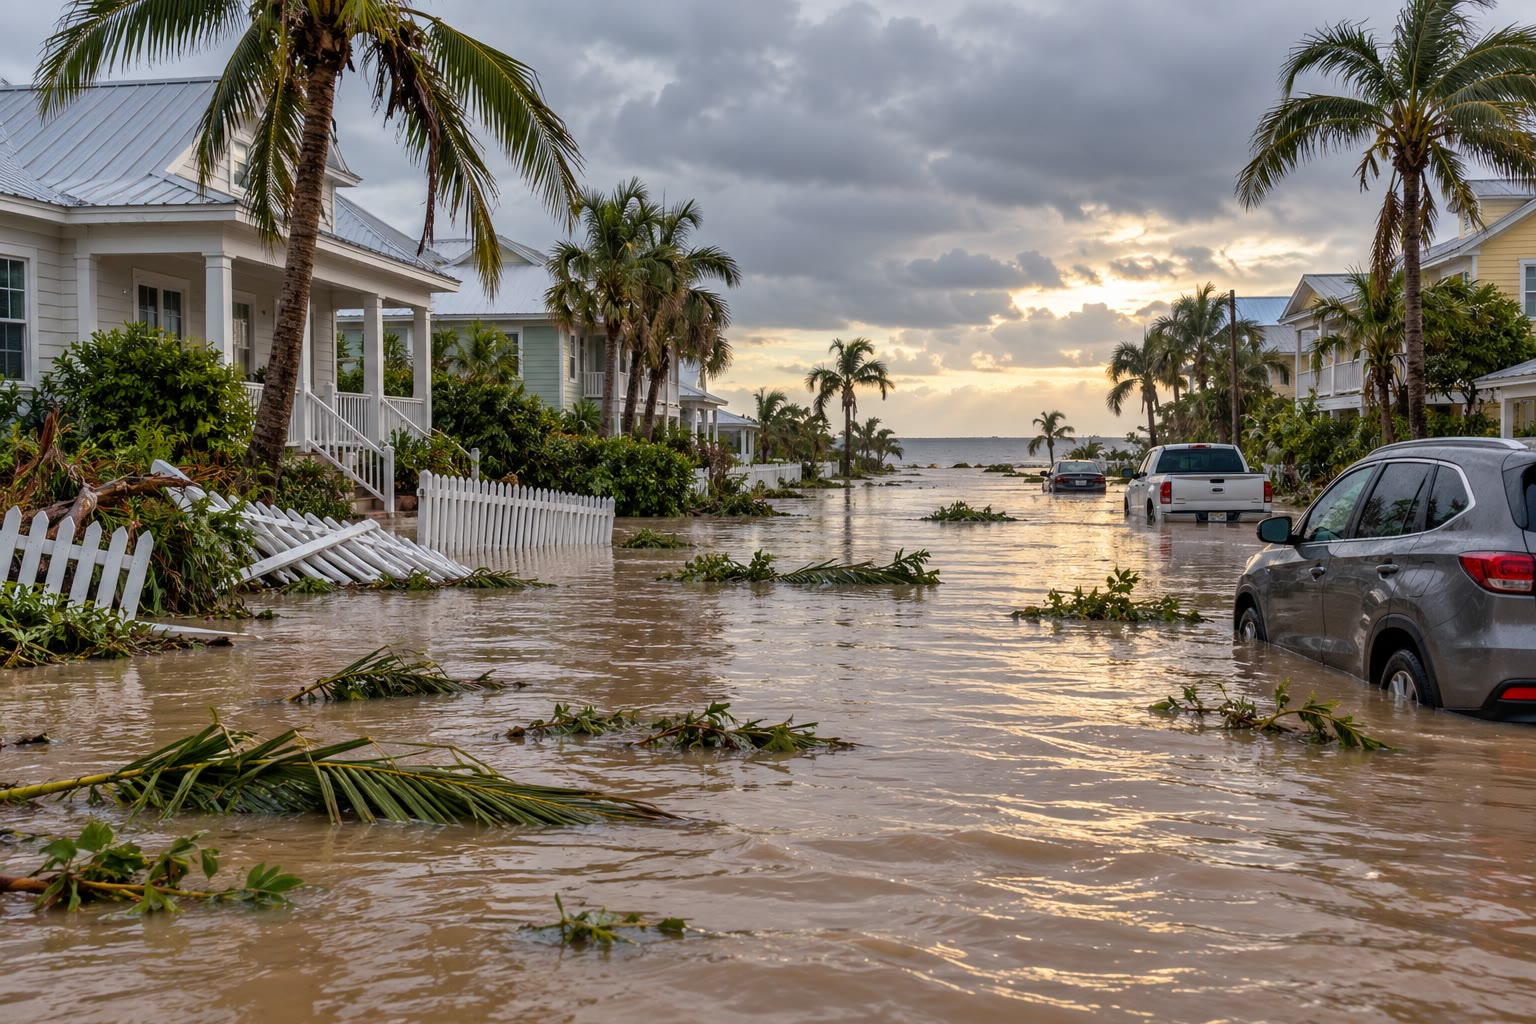
\includegraphics[width=0.7\linewidth]{images/book2/ai/g10-flooded-street.jpg}

{\small شارع ساحلي صباح اليوم التالي \omterm{def:g10:storms-and-cyclones:storm-surge}{لعرام عاصفي}: ماء البحر، ونخيل مكسور، وأسوار
ممزقة.}
\end{omfigure}

\section{تمارين}

\begin{exercise}[$\star$]\label{exo:g10:storms-and-cyclones:1}
عرّف \omterm{def:g10:storms-and-cyclones:thunderstorm}{العاصفة الرعدية} \omterm{def:g10:storms-and-cyclones:lightning}{والبرق}. وما الذي ينتج صوت الرعد؟
\end{exercise}

\begin{exercise}[$\star$]\label{exo:g10:storms-and-cyclones:2}
عرّف \omterm{def:g10:storms-and-cyclones:tropical-cyclone}{الإعصار المداري} وعينه وجدار عينه. وأين تكون رياحه على
أشدها؟
\end{exercise}

\begin{exercise}[$\star$]\label{exo:g10:storms-and-cyclones:3}
في أي فئة من \omterm{def:g10:storms-and-cyclones:scale}{سلم سافير--سيمبسون} يقع إعصار رياحه المستديمة
\num{70}~عقدة؟ و\num{120}~عقدة؟ و\num{140}~عقدة؟ وأيها من الأعاصير
الكبرى؟
\end{exercise}

\begin{exercise}[$\star$]\label{exo:g10:storms-and-cyclones:4}
تعدّ \num{9} ثوانٍ بين وميض ورعده، ثم \num{15}
ثانية للوميض التالي. ما بعد كل منهما، وهل العاصفة
تقترب؟
\end{exercise}

\begin{exercise}[$\star$]\label{exo:g10:storms-and-cyclones:5}
فسّر لماذا تكون الشجرة القائمة وحدها في حقل ملجأً خطرًا في أثناء \omterm{def:g10:storms-and-cyclones:thunderstorm}{عاصفة رعدية}،
وإلى أين ينبغي أن تذهب بدلًا منها.
\end{exercise}

\begin{exercise}[$\star\star$]\label{exo:g10:storms-and-cyclones:6}
العقدة \qty{1852}{m} في الساعة. حوّل \num{64}~عقدة و\num{137}~عقدة
إلى \unit{m/s} وإلى \unit{km/h}.
\end{exercise}

\begin{exercise}[$\star\star$]\label{exo:g10:storms-and-cyclones:7}
على الأرض 44 ومضة \omterm{def:g10:storms-and-cyclones:lightning}{برق} في كل ثانية. فكم يساوي ذلك في يوم، وفي
سنة؟
\end{exercise}

\begin{exercise}[$\star\star$]\label{exo:g10:storms-and-cyclones:8}
إعصار ضغطه في المركز \qty{935}{hPa} ومحيطه عند
\qty{1010}{hPa}. ما ارتفاع الانتفاخ الضغطي للبحر تحته؟
\end{exercise}

\begin{exercise}[$\star\star$]\label{exo:g10:storms-and-cyclones:9}
باستعمال خريطة المسارات، صِف أين تتكون \omterm{def:g10:storms-and-cyclones:tropical-cyclone}{الأعاصير المدارية} وإلى أين تتجه بعد
تكونها. ولماذا تغيب عن خط الاستواء نفسه؟
\end{exercise}

\begin{exercise}[$\star\star$]\label{exo:g10:storms-and-cyclones:10}
معادلة الخط المستقيم في مخطط الضغط والريح هي $p \approx 1031 - 1.56\,v$
($p$ بالوحدة \unit{hPa}، و$v$ بالوحدة \unit{m/s}). ما الضغط في المركز الذي تعطيه
للحد الأدنى للفئة 5، \qty{70}{m/s}؟ ولعاصفة رياحها
\qty{40}{m/s}؟
\end{exercise}

\begin{exercise}[$\star\star$]\label{exo:g10:storms-and-cyclones:11}
فسّر لماذا يضعف \omterm{def:g10:storms-and-cyclones:tropical-cyclone}{الإعصار المداري} سريعًا حين ينتقل فوق اليابسة، ولماذا يضعف فوق
الماء البارد.
\end{exercise}

\begin{exercise}[$\star\star\star$]\label{exo:g10:storms-and-cyclones:12}
سرعة الصوت في الهواء هي $\sqrt{1.4\,R\,T/M}$، حيث $R =
\qty{8.314}{J.mol^{-1}.K^{-1}}$، و$T$ بالكلفن، و$M =
\qty{0.02897}{kg/mol}$. احسبها عند \qty{0}{\degreeCelsius} وعند
\qty{30}{\degreeCelsius}. ومن أجل تأخر قدره \qty{9}{s}، بكم يختلف البعدان؟ وهل قاعدة
«\qty{3}{s} لكل كيلومتر» جيدة بما يكفي؟
\end{exercise}

\begin{exercise}[$\star\star\star$]\label{exo:g10:storms-and-cyclones:13}
يُقاس \omterm{def:g10:storms-and-cyclones:storm-surge}{عرام عاصفي} قدره \qty{4.0}{m} على ساحل في أثناء وصول إعصار ضغطه في المركز
\qty{940}{hPa} (والمحيط \qty{1010}{hPa}) إلى اليابسة. ما الجزء من العرام الذي
يعود إلى الانتفاخ الضغطي، وما الجزء الذي يعود إلى الريح؟ وإذا وصل في أثناء المد
العالي، أي \qty{1.5}{m} فوق متوسط مستوى البحر، فإلى أي ارتفاع فوق متوسط مستوى البحر
يبلغ الماء؟
\end{exercise}

\begin{exercise}[$\star\star\star$]\label{exo:g10:storms-and-cyclones:14}
\omterm{def:g10:storms-and-cyclones:tornado}{إعصار قمعي} يدور برياح سرعتها \qty{90}{m/s} على بعد \qty{100}{m} من محوره؛
وإعصار برياح سرعتها \qty{60}{m/s} في جدار عين على بعد \qty{30}{km} من
المركز. كم يستغرق الهواء ليدور دورة واحدة في كل حالة؟ قارن.
\end{exercise}

\begin{exercise}[$\star\star\star$]\label{exo:g10:storms-and-cyclones:15}
من بين \num{3888} إعصارًا مداريًا في 1980--2024، بلغ 24 منها قوة العاصفة
المدارية على بعد \qty{5}{\degree} من خط الاستواء، و414 على بعد
\qty{10}{\degree}، و121 وراء \qty{30}{\degree}. احسب النسب المئوية الثلاث. ويغطي
النطاق الواقع على بعد \qty{5}{\degree} من خط الاستواء نحو
\qty{9}{\percent} من سطح الأرض: فماذا تتوقع لو لم يكن لخط العرض أثر، وماذا
تستنتج؟
\end{exercise}

\section{مسألة: المحرك الحراري للإعصار}

\begin{problem}[{مسألة نهاية الأسبوع --- من مطر يوم إلى قدرة
الريح}]
\label{pb:g10:storms-and-cyclones:1}
% ledger: aoml:energy, nist:water-latent, earth:Rmean, ipcc:budget-toa (all results computed in figdata/grade-10/cyclones.py or from the rounded data below)
يُمطر الإعصار المتوسط \qty{1.5}{cm} في اليوم فوق دائرة نصف قطرها
\qty{665}{km}. استعمل \omterm{def:g10:earth-energy-budget:latent-heat}{حرارة كامنة} قدرها \qty{2.5}{MJ/kg}، وكثافة للماء قدرها
\qty{1000}{kg/m^3}، و\qty{86400}{s} في اليوم، وقدرة رياح الإعصار المتوسط،
\qty{1.5e12}{W}.

\medskip
\noindent\textbf{الجزء الأول --- مطر يوم.}
\begin{enumerate}
  \item احسب مساحة الدائرة.
  \item احسب حجم المطر الذي يسقط عليها في يوم.
  \item عبّر عنه بالكيلومترات المكعبة.
  \item احسب كتلته.
\end{enumerate}

\medskip
\noindent\textbf{الجزء الثاني --- الحرارة المتحررة.}
\begin{enumerate}[resume]
  \item احسب \omterm{def:g10:earth-energy-budget:latent-heat}{الحرارة الكامنة} التي يحررها في يوم تكاثف هذا
        الماء.
  \item حوّلها إلى قدرة.
  \item تمتص الأرض كلها نحو \qty{1.22e17}{W} من ضوء الشمس
        (\cref{ch:g10:earth-energy-budget}). فما الكسر منها الذي يحرره
        إعصار واحد؟
  \item متوسط ضوء الشمس الممتص \qty{240}{W/m^2}. احسب ضوء الشمس الذي
        تمتصه مساحة العاصفة وقارنه \omterm{def:g10:earth-energy-budget:latent-heat}{بالحرارة الكامنة}
        للعاصفة.
  \item ماذا تُظهر هذه المقارنة عن المكان الذي جُمعت فيه طاقة
        العاصفة؟
\end{enumerate}

\medskip
\noindent\textbf{الجزء الثالث --- من أين يأتي الماء.}
\begin{enumerate}[resume]
  \item ما كتلة الماء التي يجب أن تتبخر كل يوم لتغذية هذا المطر؟
  \item يحمل متوسط تبخر سطح الأرض
        \qty{82}{W/m^2}. فعلى أي مساحة يستطيع التبخر المتوسط أن يوفر
        \omterm{def:g10:earth-energy-budget:latent-heat}{الحرارة الكامنة} للعاصفة؟ قارن بمساحة العاصفة.
  \item باستعمال جدول المحتويات عند التشبع في
        \cref{ch:g10:why-clouds-form}، قارن الماء الذي يحمله الهواء المشبع
        عند \qty{28}{\degreeCelsius} وعند \qty{20}{\degreeCelsius}.
  \item فسّر لماذا لا تتكون \omterm{def:g10:storms-and-cyclones:tropical-cyclone}{الأعاصير المدارية} إلا فوق البحار الدافئة.
  \item فسّر لماذا تضعف فوق اليابسة.
\end{enumerate}

\medskip
\noindent\textbf{الجزء الرابع --- الريح.}
\begin{enumerate}[resume]
  \item احسب الطاقة الحركية التي تُعطى للرياح في يوم.
  \item حوّل الحد الأدنى للفئة 3، \num{96}~عقدة، إلى
        \unit{m/s} (\num{1}~عقدة = \qty{1852}{m/h}).
  \item كثافة الهواء قرب سطح البحر نحو
        \qty{1.16}{kg/m^3}. احسب الطاقة الحركية لمتر مكعب واحد
        منه يتحرك بهذه السرعة.
  \item قارن \omterm{def:g10:earth-energy-budget:latent-heat}{الحرارة الكامنة} المتحررة في يوم بطاقة الرياح في
        يوم.
  \item ما مصير بقية الحرارة المتحررة؟
  \item ما الكسر من الحرارة التي يحررها التكاثف الذي يصير ريحًا؟
\end{enumerate}
\end{problem}
